\documentclass[12pt]{article}
\usepackage{amsmath}
\usepackage{graphicx}
\usepackage{hyperref}
\usepackage[latin1]{inputenc}

\title{Trii User Manual}
\author{A project by Devs101}
\date{21/09/2018}

\begin{document}
\maketitle
\newpage
\pagenumbering{arabic}

\tableofcontents
\newpage

\section{General information}

\subsection{System Overview}
\paragraph{A skill tree is an aspect of some role-playing games, that allow custom configurations of a character's abilities. A skill tree starts with one or several base skills for either a certain class of character. After base skills, the skills branch out into either more specialized skills or just higher level skills. Trii gives the user the tools to create such a skill tree. It allows the user to create, edit, save/upload their own skill tree. This in turn can then be tested, to see how a user would progress through the skill tree.}

\subsection{System Configuration}
\paragraph{Trii is simple to access and does not require extensive hardware to be able to use it. The only requirement is that the user has Google Chrome and Internet access for the initial loading of Trii. Trii itself is hosted on a GitHub server and users that connect to it will then automatically allow Trii to be saved locally and can then be used offline if needed.}

\begin{figure}
  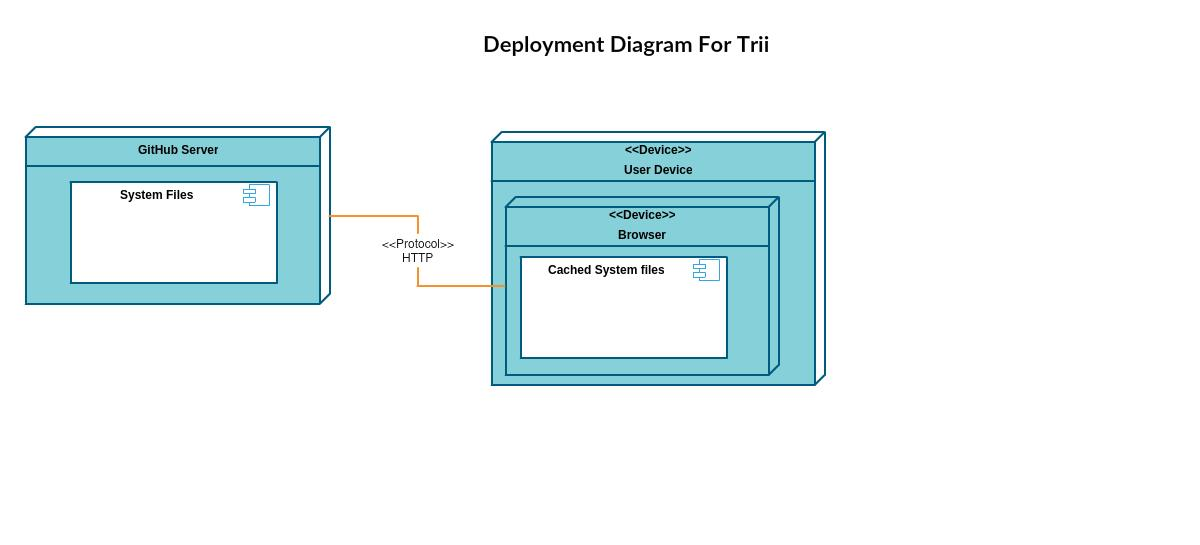
\includegraphics[width=\linewidth]{deployment.jpg}
  \caption{The Deployment diagram.}
  \label{fig:deployment}
\end{figure}

\newpage
\subsection{Installation}
\begin{enumerate}
	\item Google Chrome can be downloaded from www.google.com/chrome/
	\begin{enumerate}
    	\item Once the site has loaded press download chrome.
      \item Chrome will then be downloaded, once it is done click on the downloaded file.
      \item Follow the prompts, Google Chrome will then download the remaining files.
      \item After the installation Chrome can be accessed via the desktop, Start menu or Installed location. (Mobile users will either have it default on their phone or will be able to get it via the app store.)
    \end{enumerate}
	\item The software(Trie) can be accessed at https://dolan212.github.io.
	\item After the initial access Trii will be saved on the user's local storage allowing for quick access on and offline.
	\item On mobile versions Trii will create a shortcut automatically, this can be found in the user's app list.
	\item Trii is then ready for use.
\end{enumerate}

\newpage
\section{Getting started}
\subsection{Accessing Trii}
\begin{enumerate}
  \item Launch Google Chrome.
  \item Once Google Chrome has opened type https://dolan212.github.io in the navigation bar located at the top and press enter.
  \item When the site has loaded the following image below is what should be displayed. Press "GET STARTED" to access Trii.
  \item To close Trii the user can close Google Chrome, as displayed in the second image below.
\end{enumerate}


\begin{figure}
  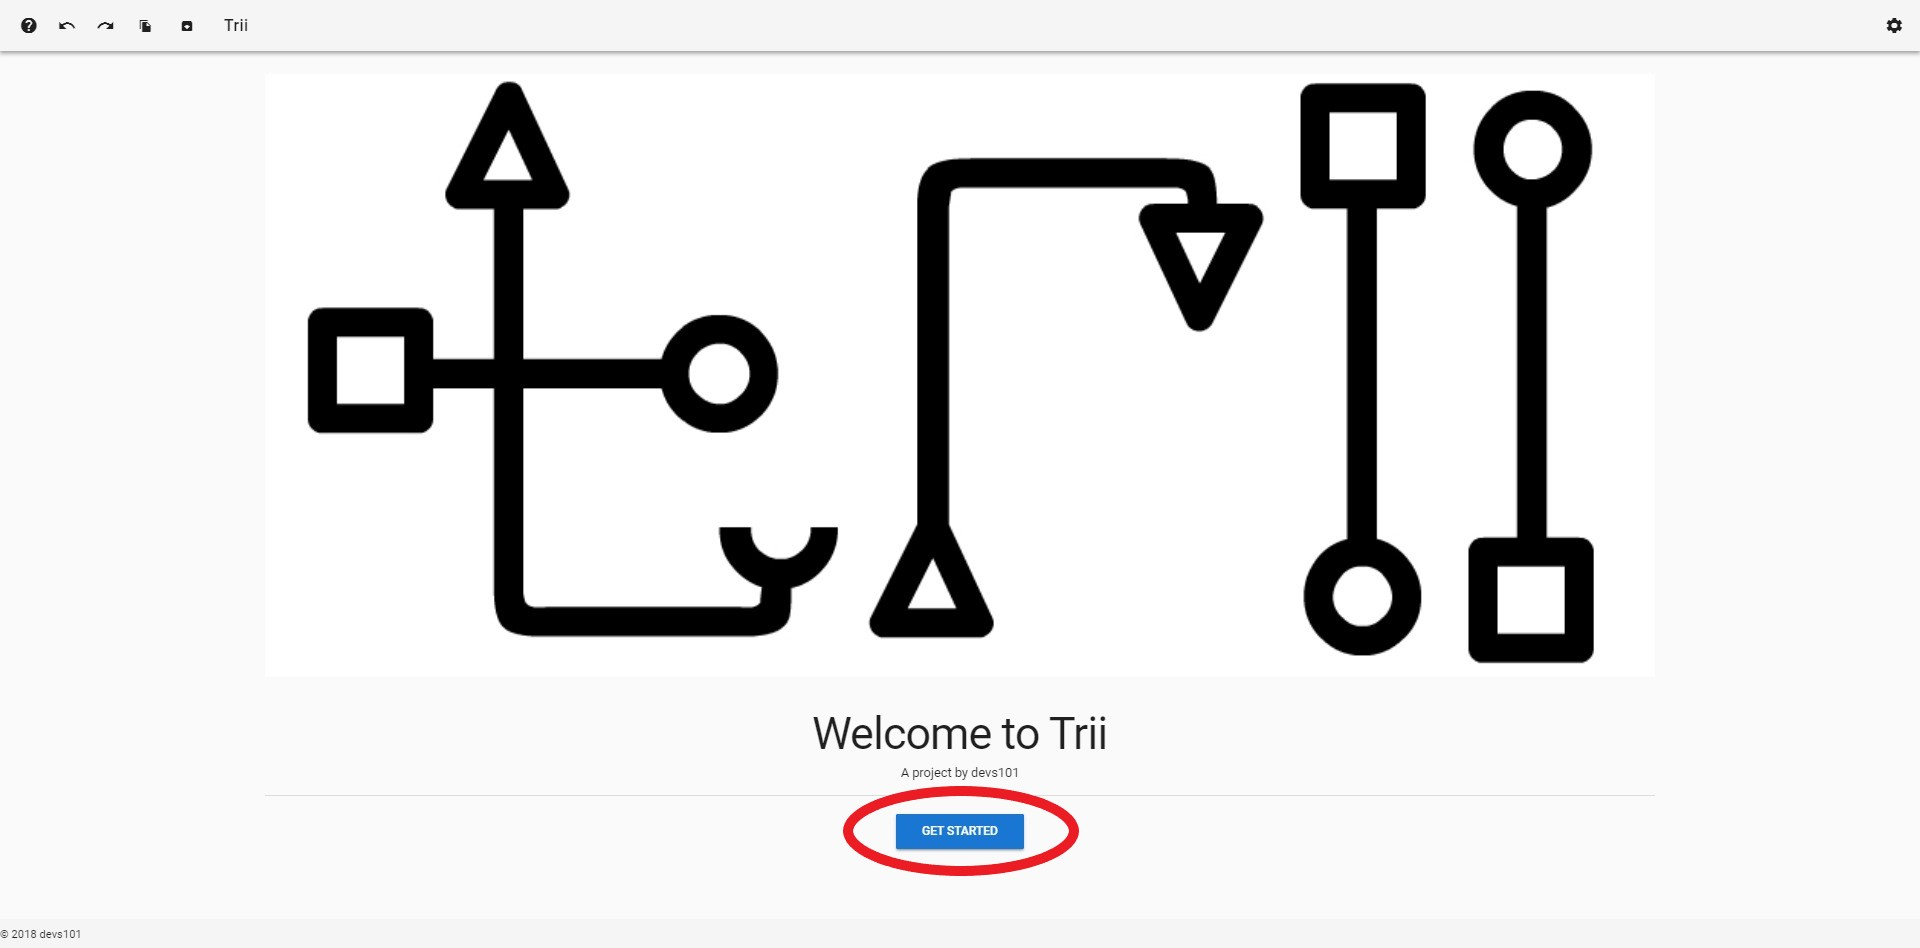
\includegraphics[width=\linewidth]{homepage.jpg}
  \caption{The Home Page of Trii.}
  \label{fig:homepage}
\end{figure}

\begin{figure}
  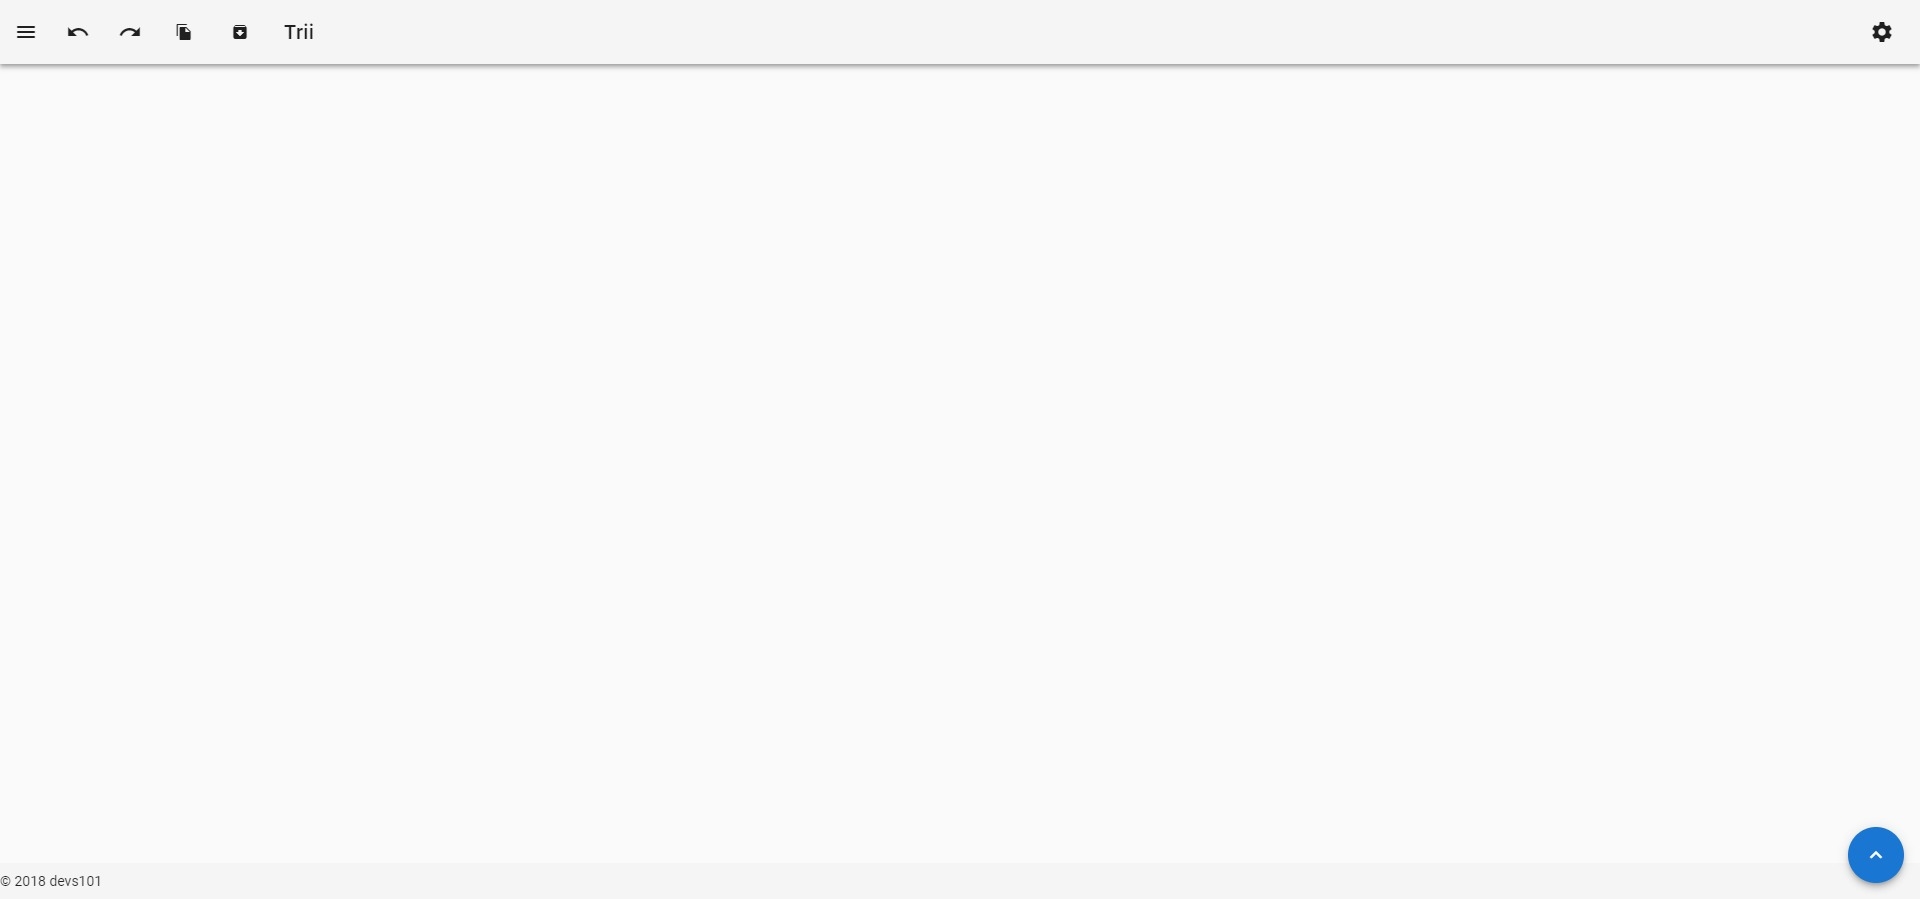
\includegraphics[width=\linewidth]{startclose.jpg}
  \caption{Get started and how to close.}
  \label{fig:startclose}
\end{figure}

\newpage
\section{Using the system}
\subsection{The Basics}
\paragraph{In this section the basic layout will be discussed. This is just to help the user familiarize themselves with the layout with Trii. The following list will be accompanied by a few images to help with a visual guide.}

\begin{enumerate}
	\item Action bar
	\begin{enumerate}
    	\item Add Skill
      	\item Edit Skill
      	\item Delete Skill
 	\end{enumerate}
  
  \begin{figure}
    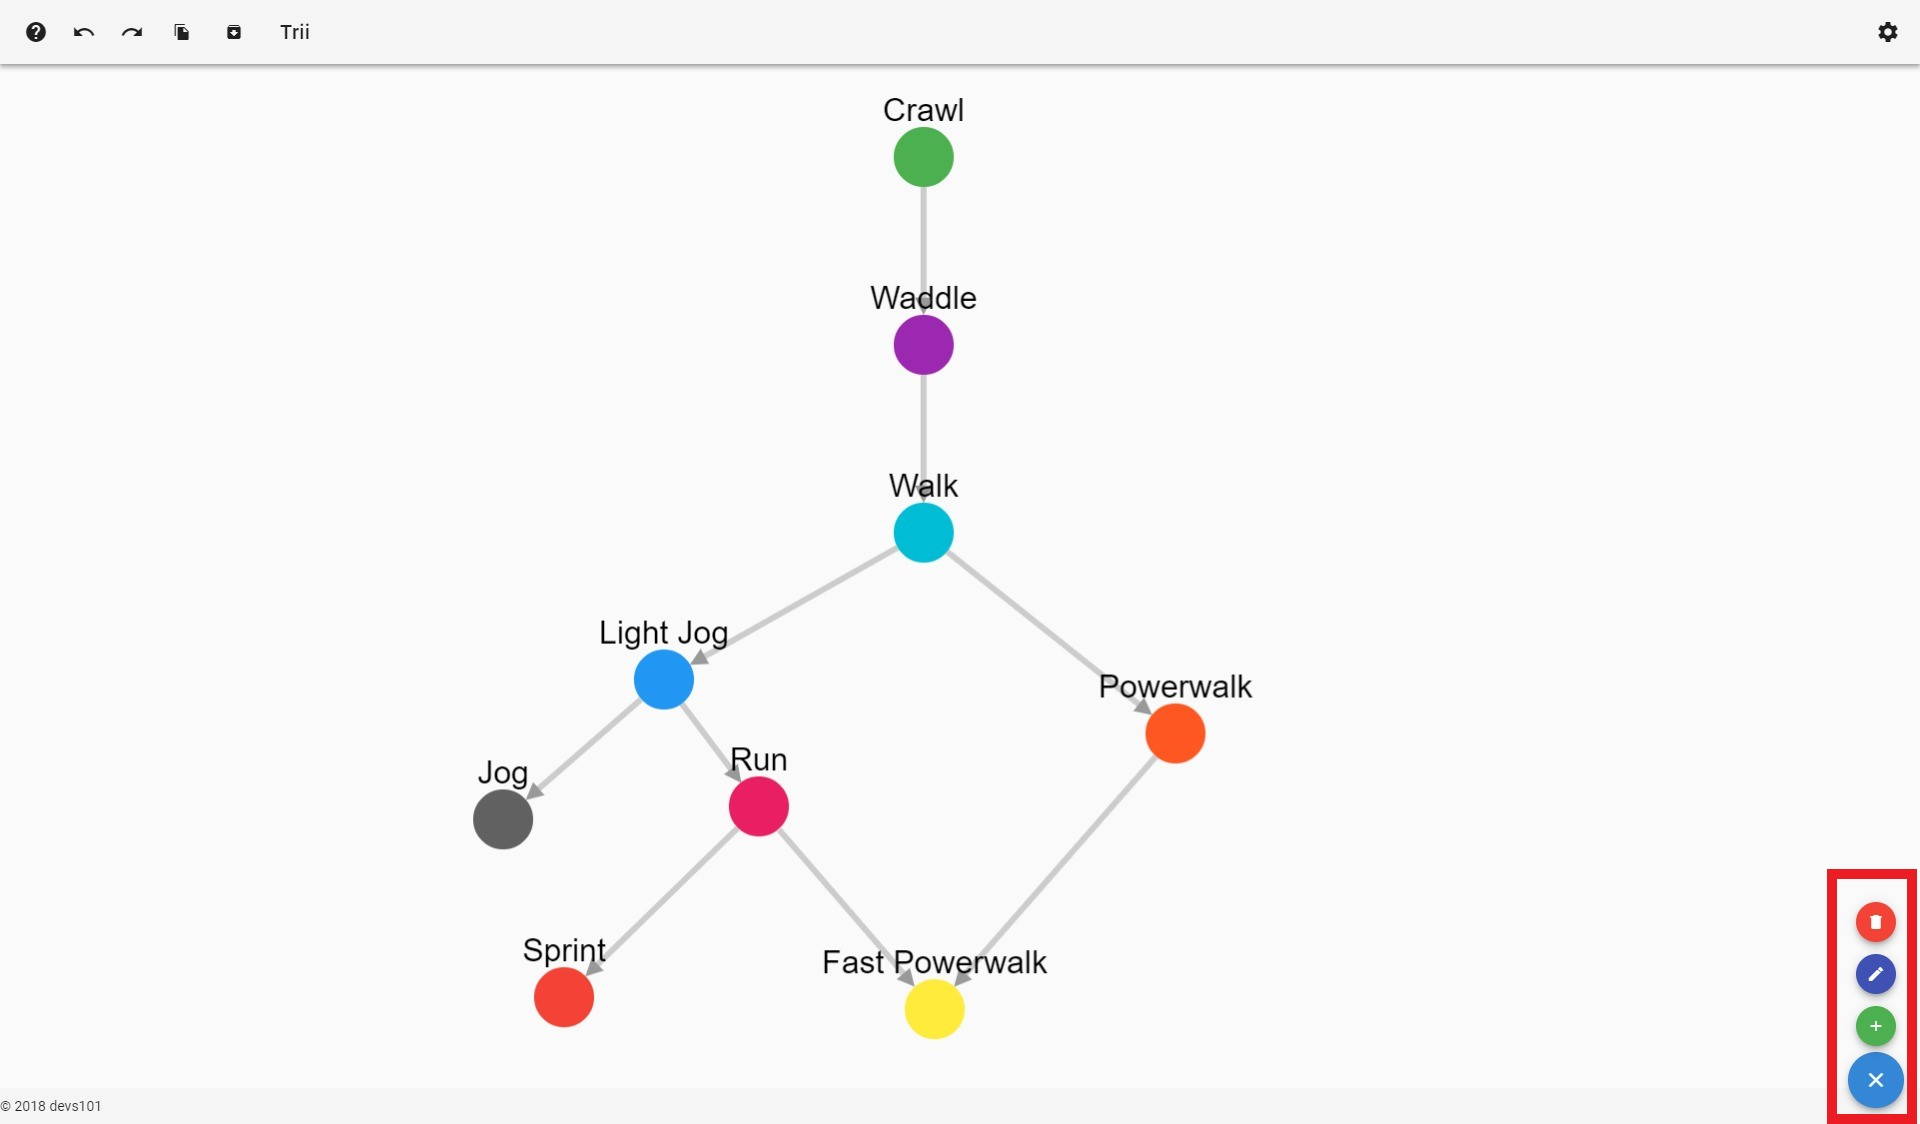
\includegraphics[width=\linewidth]{actionbar.jpg}
    \caption{The Action Bar.}
    \label{fig:actionbar}
  \end{figure}

  
  \item Toolbar
  \begin{enumerate}
    	\item Undo
      \item Redo
      \item Copy
      \item Paste
  \end{enumerate}
  
  \begin{figure}
    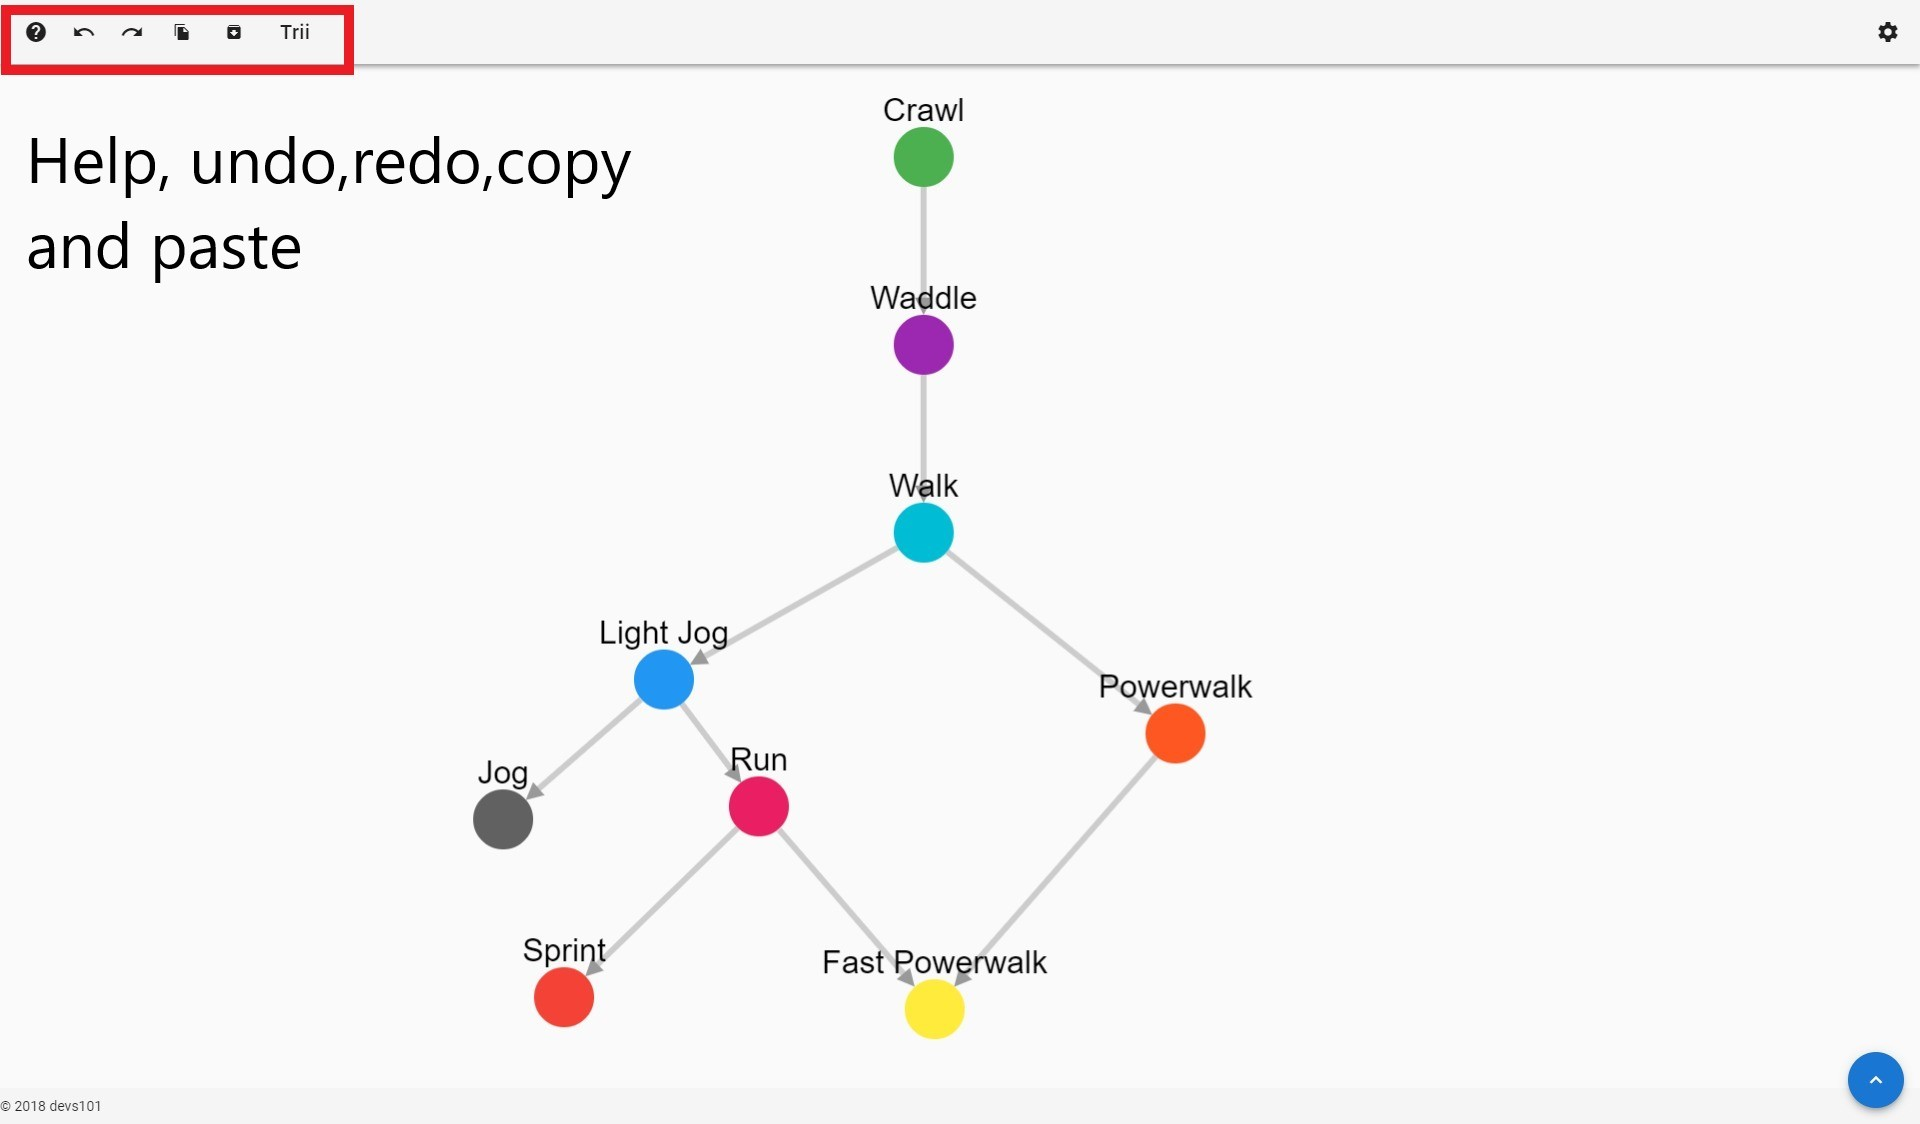
\includegraphics[width=\linewidth]{toolbar.jpg}
    \caption{The Toolbar}
    \label{fig:toolbar}
  \end{figure}
  
  \item Settings
  \begin{enumerate}
    	\item Clear Tree
      \item Auto Layout
      \item Import Skill Tree
      \item Export Skill Tree
  \end{enumerate}
  
  \begin{figure}
    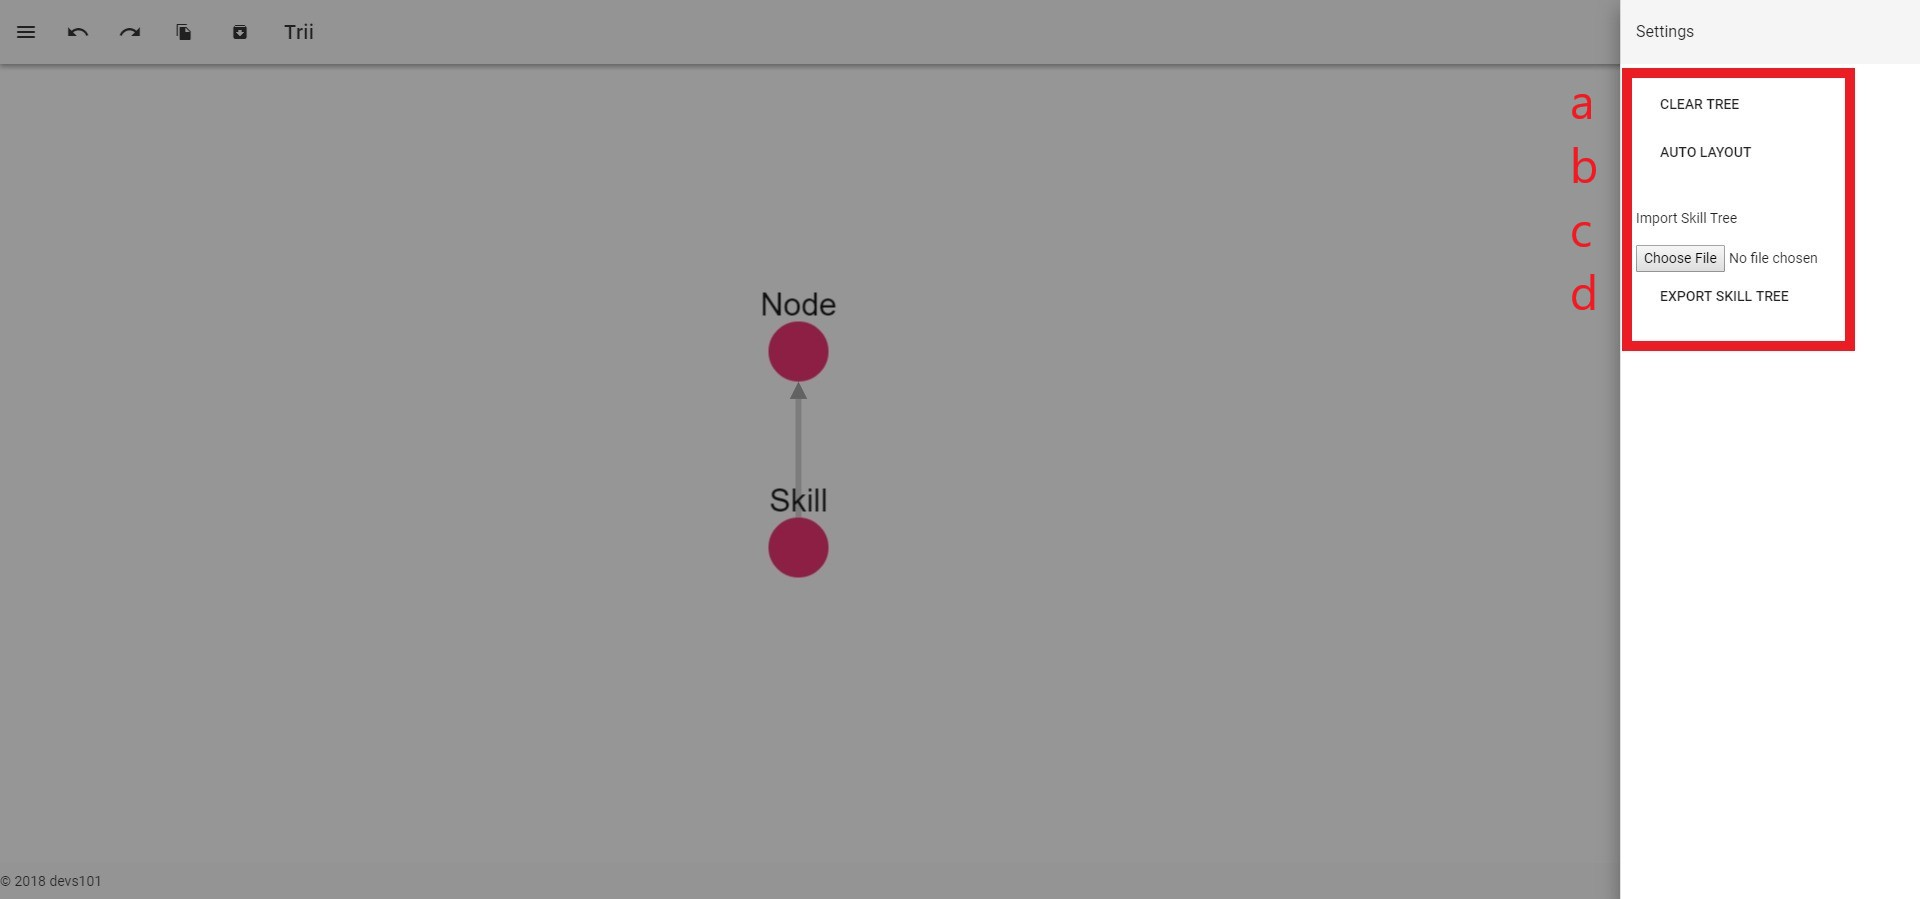
\includegraphics[width=\linewidth]{settings.jpg}
    \caption{Settings for Trii.}
    \label{fig:settings}
  \end{figure}
  
\end{enumerate}

\newpage
\subsection{Creating a Tree}
\paragraph{Creating a Tree will involve adding Nodes and Edges}

\paragraph{Adding a Node:}

\begin{enumerate}
	\item To add a Node press the Add Skill button.
	\item A popup will appear and will prompt you for a name for the skill. Enter a name and press the ADD button.
	\item If you do not wish to add a skill simply press the close button.
	\item A new node will appear on the screen.
\end{enumerate}

\paragraph{Adding an Edge:}

\begin{enumerate}
	\item To add an Edge you require at least 2 Nodes/Skills.
	\item To add an edge between 2 nodes select a node.
	\item The selected node will now have a yellow outline to indicate that it is selected.
	\item Press the Edit Skill button in the Action bar.
	\item Press the Add Rule button.
	\item A new window will appear with 2 dropdown menus.
	\item For the first dropdown select Dependency, for the second choose the node you want it connected to.
	\item Press save, a new edge will be created between the 2 nodes.
\end{enumerate}

\paragraph{Editing the Node/Skill name:}
\begin{enumerate}
	\item Select a Node.
	\item Press the Edit Skill button in the Action bar.
	\item Edit the name under the Skill Name edit bar.
\end{enumerate}

\paragraph{Adding a description to the Skill/Node:}
\begin{enumerate}
	\item Select a Node.
	\item Press the Edit Skill button in the Action bar.
	\item Add your description in the Description edit bar and press save.
\end{enumerate}

\paragraph{Editing the Node/Skill name:}
\begin{enumerate}
	\item Select a Node.
	\item Press the Edit Skill button in the Action bar.
	\item Select a color from the dropdownlist.
\end{enumerate}

\paragraph{Setting the required Level:}
\begin{enumerate}
	\item Select a Node.
	\item Press the Edit Skill button in the Action bar.
	\item Press the Add Rule button.
	\item A new window will appear with 2 dropdown menus.
	\item For the first dropdown select Level, for the second choose a value you wish to set the required level.
	\item Press Save.
\end{enumerate}

\paragraph{Setting the required Skill Points:}
\begin{enumerate}
	\item Select a Node.
	\item Press the Edit Skill button in the Action bar.
	\item Press the Add Rule button.
	\item A new window will appear with 2 dropdown menus.
	\item For the first dropdown select Skill Points, for the second choose a value you wish to set the required skill points.
	\item Press Save.
\end{enumerate}

\paragraph{Deleting a Node/Skill:}
\begin{enumerate}
	\item Select a Node.
	\item Press the Delete Skill button in the Action bar.
	\item The node/skill will be deleted.
	\item Multiple nodes can be deleted at once if more than one node is selected.
\end{enumerate}

\paragraph{Deleting an Edge:}
\begin{enumerate}
	\item Select a Node.
	\item Press the Edit Skill button in the Action bar.
	\item Locate the Dependancy you wish to remove.
	\item Simply click the x button.
	\item Press save, the edge will be removed.
\end{enumerate}

\subsection{Using the Toolbar}
\paragraph{The toolbar has a few helpful buttons to help during the creation of the tree.}

\paragraph{Undo:}
\begin{enumerate}
	\item Press the undo button to roll back to a previous version of the tree.
\end{enumerate}

\paragraph{Undo:}
\begin{enumerate}
	\item Press the redo button to get back what was lost from undo.
\end{enumerate}

\paragraph{Redo:}
\begin{enumerate}
	\item Press the redo button to get back what was lost from undo.
\end{enumerate}

\paragraph{Copy:}
\begin{enumerate}
	\item Select a Node/Skill.
	\item Press the Copy button.
	\item Multiple nodes/skills can be copied.
\end{enumerate}

\paragraph{Paste:}
\begin{enumerate}
	\item Press the Paste button.
	\item All nodes/skills that have been coppied will be pasted on the screen.
\end{enumerate}

\subsection{Settings}
\paragraph{The Settings bar allow for some more options regarding the tree as a whole. Import and export functionality for the tree itself, it will be in a JSON format. Clear Tree to clear everything. Auto Layout to reorganize the Tree.}

\paragraph{Clear Tree:}
\begin{enumerate}
	\item Press the Clear Tree button.
	\item All nodes/skills and edges will be deleted.
\end{enumerate}

\paragraph{Auto Layout:}
\begin{enumerate}
	\item Press the Auto Layout button.
	\item The tree will reorganize itself to make it easier to view, The nodes and skills will move apart a certain distance and take form of a tree structure.
\end{enumerate}

\paragraph{Import:}
\begin{enumerate}
	\item Press the Import button.
	\item A file browser will pop up, navigate to the .json file you wish to import. Select the file.
	\item The file will be read in and the Skill Tree will be displayed.
\end{enumerate}

\paragraph{Export:}
\begin{enumerate}
	\item Press the Export button.
	\item A window will pop up with a prompt for the file name.
	\item Enter a name for the file.
	\item Press Export or Close if you don't want to download the file.
	\item The file will then be downloaded via the chrome browser and can be located in the downloads folder (Same location for mobile users).
\end{enumerate}

\newpage
\section{Troubleshooting}
\subsection{Accessing Trii}
    \begin{enumerate}
    	\item Make sure you have internet access.
      \item Make sure you entered the correct address in the top bar of Google Chrome
      \item Refresh the page if it did not load correctly.
    \end{enumerate}
    
\subsection{Mistakes made in try}
    \begin{enumerate}
    	\item Make use of the Redo/Undo buttons.
      \item You can always start from scratch if you so wish.
      \item Always export progress for in case something happens (Errors, Unintentional closure of Trii, Loss of power, etc.)
    \end{enumerate}
    
\end{document}    


